\documentclass[a4paper, twoside, 11pt]{article}
\usepackage[margin=1.5cm]{geometry}
\usepackage[]{xcolor}
\usepackage{cite}
\usepackage{graphicx}
\usepackage{listings}
\usepackage{float}
\usepackage{amsmath}

\usepackage{hyperref}

\hypersetup{
    colorlinks=true,
    linkcolor=blue,
    filecolor=magenta,      
    urlcolor=cyan,
}

\lstset{frame=tb,
  language=Java,
  aboveskip=3mm,
  belowskip=3mm,
  showstringspaces=false,
  columns=flexible,
  basicstyle={\small\ttfamily},
  numbers=none,
  numberstyle=\tiny\color{gray},
  keywordstyle=\color{blue},
  commentstyle=\color{dkgreen},
  stringstyle=\color{mauve},
  breaklines=true,
  breakatwhitespace=true,
  tabsize=3
}

\definecolor{dkgreen}{rgb}{0,0.6,0}
\definecolor{gray}{rgb}{0.5,0.5,0.5}
\definecolor{mauve}{rgb}{0.58,0,0.82}

% define the title
\author{L. ~Towell,\\ Student No: 201383538}

%defines the title
\title{Assignment 1\break Brute Force Attack Estimation}

\begin{document}
	%generate the title
	\maketitle

\maketitle
\begin{center}
Code repository: \href{https://github.com/luketowell/COMP522-Assignment2}{COMP522-Assignment 2}
\end{center}

\section{Comparison of methods for message authentication}
\subsection{Hash-functions}
\subsubsection{}
\subsection{RSA + SHA1 method}
\subsection{DSA method}
\subsection{HMAC-SHA256 method}


\section{Diffie-Hellman with 4 parties}
\subsection{Design for the Diffie-Hellman Protocol}
Following the principles of the Diffie Hellman Protocol means that in order
to read the messages that are being transmitted every party needs to know the
public key of all of the other members in the network in order to generate a shared secret key.

The process is largely the same when more parties are added however because more parties have been added it means that more keys need to be generated and shared. Each party starts the process by using the shared prime number ($q$) and the shared primitive root ($\alpha$ of $q$)

Each key then generates their public keys using an random integer that they have generated. \\
$Y_A = \alpha^{X_A}$ mod q \\
$Y_B = \alpha^{X_B}$ mod q \\
$Y_C = \alpha^{X_C}$ mod q \\
$Y_D = \alpha^{X_D}$ mod q \\

The above keys are then shared among all members of the network
then the following calculations are performed in order to calculate the secret Keys\\
A calculates K = $(Y_{BCD})^{X_A}$ mod q \\
B calculates K = $(Y_{ACD})^{X_B}$ mod q \\
C calculates K = $(Y_{ABD})^{X_C}$ mod q \\
D calculates K = $(Y_{ABC})^{X_D}$ mod q \\




\subsection{Implementation of the Protocol with 4 Parties}
\subsection{Conclusion}
As can be seen from the code in \textit{Appendix D. }I have had to exchange all of the keys amongst each of the members in the network. I have done this through multiple iterations (phases) of the network in order
for everyone within the network to have all of the keys needed to successfully generate a shared secret key for decoding messages that are sent. 
\textit{figure 1.} shows the iteration cycle of how keys are exchanged over multiple iterations.

\begin{figure}[H]
	\centering
	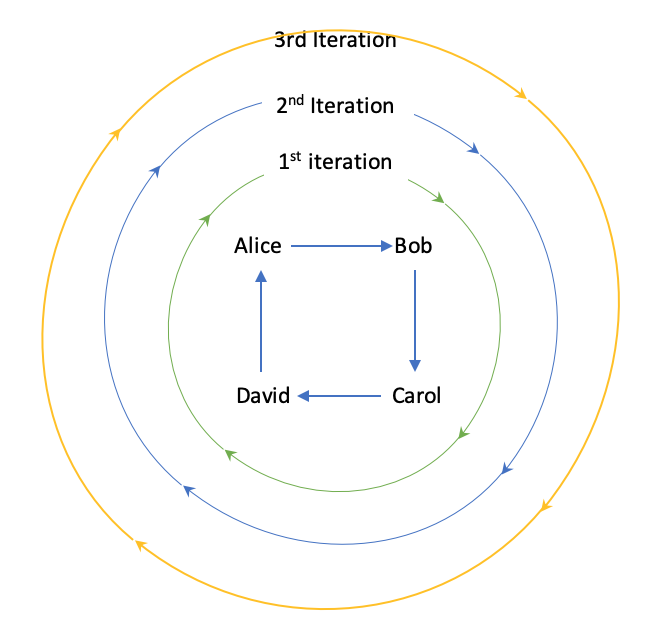
\includegraphics[scale=0.8]{Images/KeyIteration.png}
	\caption{Diagram of how keys are passed between members of network.}
\end{figure}

\textit{Table 1.} below details how the keys are gathered. In iteration 0 the only keys that each
members have are their own however as we iterate around the network the keys are gathered until every member
has every other members public keys which enables them to be able to decode the messages that have been encrypted with private keys. 

\begin{center}
	\begin{tabular}{ |c|l|l|l|l| } 
	 \hline
	 \multicolumn{1}{|c|}{}& \multicolumn {4}{|c|}{Public Keys held by network members} \\
	 \hline
   N & Alice & Bob & Carol & David \\
   \hline
   0 & A & B & C & D \\
   1 & AD & BA & CB & DC \\
   2 & ADC & BAD & CBA & DCB \\
   3 & ADCB & BADC & CBAD & DCBA \\
	 \hline
	\end{tabular}
\end{center}


\end{document}